\documentclass[sigconf]{acmart}
\usepackage[utf8]{inputenc}
\usepackage[english]{babel}

% Figures
\usepackage{epsfig}
\usepackage{epstopdf}
\usepackage{subfigure}

% Math
\usepackage{amsmath}
\usepackage{mathtools}
\newcommand{\pluseq}{\mathrel{+}=}
\newcommand{\asteq}{\mathrel{*}=}
\DeclareMathOperator*{\argmin}{arg\,min}
\DeclareMathOperator*{\argmax}{arg\,max}
\newcommand\bigforall{\mbox{\Large $\mathsurround0pt\forall$}} 

% Algorithms
\usepackage{algorithm}
\usepackage{algorithmic}
\renewcommand{\algorithmicrequire}{\textbf{Input:}}
\renewcommand{\algorithmicensure}{\textbf{Output:}}

% Table
\usepackage{multirow}
\usepackage{colortbl}
\definecolor{kugray5}{RGB}{224,224,224}
\usepackage{rotating}

\usepackage{cleveref}

\newcommand{\moedit}[1]{\textcolor{cyan}{\emph{[Mohammad: #1]}}}
\newcommand{\csedit}[1]{\textcolor{magenta}{\emph{[Cyrus: #1]}}}

\begin{document}
\title{An On-line Truthful and Individually Rational\\Pricing Mechanism for Ride-sharing}
\author{Mohammad Asghari}
\affiliation{%
  \institution{University of Southern California}
  \city{Los Angeles}
  \state{CA}
  \country{USA}
}
\email{masghari@usc.edu}
\author{Cyrus Shahabi}
\affiliation{%
  \institution{University of Southern California}
  \city{Los Angeles}
  \state{CA}
  \country{USA}
}
\email{shahabi@usc.edu}

\begin{abstract}
Ride-sharing has the potential of addressing many socioeconomic challenges related to transportation. The rising popularity of ride-sharing platforms (e.g., Uber, Lyft, DiDi) in addition to the emergence of new applications like food delivery and grocery shopping which use a similar platform,  calls for an in-depth and detailed evaluation of various aspects of this problem.\\
Auction frameworks and mechanism design, have been widely used for modeling ride-sharing platforms. A key challenge in these approaches is preventing the involving parties from manipulating the platform for their personal gain which in turn, can result in a less satisfactory experience for other parties and/or loss of profit for the platform provider. We introduce a latent space transition model for ride-sharing platforms which drivers can exploit and predict the future supply of the drivers (i.e., available drivers) to their own advantage. Following, we propose a pricing model for ride-sharing platforms which is both truthful and individually rational based on Vickery auctions and show how we can manage the loss of revenue in this approach. We compare our predicting model and pricing model with competing approaches through experiments on New York City's taxi dataset. Our results show that our model can accurately learn the transition patterns of people's ride requests. Furthermore, our pricing mechanism forces drivers to be truthful and takes away any unfair advantage the drivers can achieve by bidding untruthfully. More importantly, our pricing model forces truthfulness without sacrificing much profit unlike what is typical with second-price auction schemes.
\end{abstract}

\copyrightyear{2017}
\acmYear{2017}
\setcopyright{acmcopyright}
\acmConference{SIGSPATIAL'17}{November 7--10, 2017}{Los Angeles Area,
CA, USA}\acmPrice{15.00}\acmDOI{10.1145/3139958.3139991}
\acmISBN{978-1-4503-5490-5/17/11}
\maketitle

\vspace{-0.15in}
\section*{Categories and Subject Descriptors}
\vspace{-0.025in}
H.3.5 [\textbf{Information Storage and Retrieval}]: Online Information Services-\textit{Commercial services}

\vspace{-0.1in}
\section*{Keywords}
\vspace{-0.025in}
Ride-sharing, Revenue Maximization, Spatial Crowdsourcing

\section{Introduction}
\label{sec:intro}
%TO-DO lists:
%\begin{itemize}
%	\item Problem definition: define driver profile, rider profile and our price model.
%	
%	\item Define our objective functions (i.e., maximize extra profit), and differentiate it with other optimization goal (e.g., minimize extra distance). 
%	%Given a rider and a driver with their profiles, calculate the cost of accepting the rider. 
%	
%	\item Introduce overall framework, and describe our auction-based mechanism.
%	
%	\item Properties of our framework in both local setting and global setting. In the local setting, show that we will get the same profit as the centralized setting. In the global setting, show that our technique can achieve certain approximation ratio compared with the global optimal (or upper bound of global optimal),  or vice verse we will suffer from certain degenerated cases.
%	
%	\item Optimizations: a) Maintain coarse-grained hierarchic index (adaptive grids, quad-tree), b) maintain novel shortest path index which is fine tuned for ride-sharing applications c) batch processing rider requests (single round bidding v.s. multi-round bidding).
%	
%\end{itemize}

%%%%%% 1. background information
% Ridesharing becomes popular recently because it has potential to match riders with similar itineraries and time schedules, and to bring significant benefits to individual users and the city as a whole. 

Real-time ride-sharing, as an alternative transportation service, alleviates traffic congestion and decreases auto emissions. With the emergence of many commercial platforms (e.g., Uber and Lyft), which automatically match drivers and riders on-the-fly, real-time ride-sharing becomes more and more popular. According to~\cite{uberpool}, millions of trips have been taken on UberPool since its launch at August 2014, and thousands of passengers take it five times a week during commuting hours. Enabled by the development and technology advances of smart phones and location-based services, ride-sharing platforms typically operate as follows: (1) Riders and drivers can join the platform via their smart phones, (2) a rider can submit a request, which consists of the pick-up and drop-off points, to the platform, (3) once a new request is received, the platform determines a driver (even en-route) to pick up the rider, (4) when the trip is completed, the platform calculates the rider's fare and the driver's income. With these platforms, riders can share a vehicle with reduced trip cost while enjoying fast and convenient transportation.

%%%%%% 2. explain the challengs and the detour of ridesharing......
Many challenges exist to enable such real-time ride-sharing platforms. From a business point of view, the platform provider (e.g., Uber) seeks to maximize its own profit. However, higher profits should not be at the cost of either charging passengers more or paying drivers less than what would compromise participation and retention due to no monetarily incentive for either parties. Consequently, the design of a fair pricing model becomes an essential business strategy. This is particularly important in cases of carpooling where riders share their ride with other riders. Even though carpooling reduces the riders' cost, it incurs extra distance (i.e., detour) for riders. While each rider's fare should be discounted as a function of the length of the detour, the driver should be rewarded more as the total travel distance is increased due to all detours. Furthermore, different users (i.e., riders and drivers) might value their time differently. Therefore, a fair pricing model should be available to both riders and drivers to express, for a certain amount of detour, how much discount or compensation they expect. Finally, in addition to fair pricing scheme for riders and drivers, the model should account for the provider's revenue as well.

The second challenge of a ride-sharing platform is to process incoming requests in real-time. This involves two different tasks: i) checking which drivers can add the new requests (new pick-up and drop-off locations) to their current trip without violating the constraints of that trip (i.e., scheduling) and ii) selecting the best driver among those who can serve the new request (i.e., matching). Processing the schedule of potentially thousands of drivers to check if they can accommodate a new request, with the additional task of matching their pricing profile with the incoming rider's profile, becomes computationally intensive. Therefore, the design of an efficient and scalable algorithm that assigns riders to drivers with a fair pricing model while maximizing the provider's revenue, is very challenging.


%First, the framework should consider the conflicting interests of different users (i.e., riders and drivers) and platform providers (e.g., Uber). For example, riders would like to arrive at their destination as quick and cheap as possible, whereas drivers and platform providers would like to maximize their profits. Although ride-sharing can reduce the cost of riders by sharing similar itineraries, it also incurs extra travel distance (i.e., detour). Ideally, riders are expected to be compensated for their detour, while drivers are expected to earn more profit. These factors makes the design of a fair pricing scheme (i.e., the fares and incomes) that satisfies the requirements of both riders and drivers even more complex. Secondly, because the riders requests are generated on-the-fly, the framework should decide the matching drivers (even en-route) at a short amount of time. Therefore, the design of an efficient framework that match riders and drivers, with a fair pricing scheme that provides incentives for all participants becomes a distinguishing business strategy. 

%%% 3. show the shortcomings of existing work and how they fail to address the challenge
The majority of previous studies~\cite{Ota15, Cici15, Cao15, PelzerITS15} focus on improving the efficiency of on-the-fly assignment with the objective of minimizing the total travel distance of drivers. In particular, in existing studies a new request is assigned to a driver who can fit the request in his schedule with the least amount of increase in the total traveled distance. However, minimizing drivers' total travel distance is not always equivalent to overall shorter trips for riders. Consequently, when assigning a new request, the driver who would incur the minimum increase in total travel distance is not necessarily the most cost effective option. To illustrate, suppose driver $a$ has two passengers on board and driver $b$ has only one. To serve an incoming request, \textit{a}'s incurred detour is 2 miles while for $b$ the detour is 3 miles. Even though $a$'s detour is shorter, the platform owner has to compensate both passengers of $a$ for 2 miles (a total of 4 miles) while in the case of $b$ it has to compensate only one passenger for a total of $3$ miles. In addition, from the riders' perspectives, in the first scenario two riders incur extra detour while in the second only one rider incurs an extra detour.  Few studies~\cite{Ma13,Ma15} consider a pricing model by defining monetary incentives for riders and drivers. In \cite{Ma13}, a pricing model is introduced where instead of being compensated, a rider can potentially end up being penalized for longer detours by paying a higher fare. Ma et. al.~\cite{Ma15} overcomes the unfairness issue in \cite{Ma13} to some extent. Even though, a new rider can incur detour in his trip, their model only compensates riders that are already on board. In addition, since this model is targeted for a different application, the notion of revenue fails to provide any incentive for the platform provider. Furthermore, in all previous studies~\cite{Ma13,Huang14,Ma15}, a centralized server is responsible for matching and scheduling incoming requests. Most of these studies utilize a spatiotemporal index to enable matching, i.e., narrowing down the number of potential drivers who can serve an incoming request. With thousands of drivers in the system, even after applying the spatial index, the centralized server still needs to perform scheduling and profile matching for all the candidate drivers. We show that with large number of drivers, these frameworks fail to process new requests in real-time (\cref{subsec:exprp}) and hence not scalable.


%in In \cite{Ma13}, a pricing model is introduced where instead of being compensated, a rider can potentially end up being penalized for longer detours by paying a higher fare. 

%In a recent study \cite{Ma15}, the pricing model overcomes the unfairness issue in \cite{Ma13} to some extent. Since riders can value their time differently, It also allows riders to accept/reject ride-sharing requests based on the amount they will be compensated for the incurred detour. However, drivers can similarly value their time different from each other. The pricing model in \cite{Ma15} does not provide any means for drivers to specify their monetary expectations for participating in the system. Furthermore, since this model only tends to divide the cost of the ride among riders, the notion of revenue is left out and it does not provide any incentive for the platform provider.


%%% 4. explain our pricing model, and provide more intuition of better service quality.
To address aforementioned challenges, in this paper, we introduce an Auction-based Price-Aware Real-time (\textit{APART}) ride-sharing framework. We propose a general and versatile pricing model that allows both riders and drivers to set their monetary expectations for participating in ride-sharing based on their predefined profiles. Specifically, each rider's profile defines the expected discount ratio for the detours incurred by ride-sharing. For example, one rider can express that he is willing to accept a 10 mile detour for 30\% discount. On the other hand, each driver's profile defines the expected cost in terms of his total travel distance and time. The model also accounts for the revenue of the platform provider. Consequently, our objective is to maximize the revenue of the ride-sharing framework while satisfying various temporal and monetary constraints of all users. APART is price-aware because a new request is assigned to a driver which generates the highest profit. Since our pricing model is designed to compensate riders for detours, the most profitable choice is also the one where \textit{riders} incur the least amount of detour, hence better service quality. Finally, APART also maximizes the revenue of the provider by increasing the service rate (throughput) in the system through engaging available drivers more effectively to serve more requests.


% With our price scheme, our objective is to maximize the total profit of the ridesharing platform, while satisfying the constraints of both riders and drivers.

% Because our pricing model compensates riders for longer trips, in order to maximize the profit, our framework reduces the detour of passengers and hence, providing better service quality. 

%We define a fair price model, which is flexible and general. The profiles are served to xxx. The constraints of are expressed as profiles. Given a user and rider profile, the fare and cost of xxx can be automatically derived from their profiles and other constrains. 

%%% 5. explain our framework
To efficiently assign riders to the candidate drivers, we introduce a distributed auction-based framework. With our framework, APART, the server broadcasts a new request to a set of candidate drivers and the mobile app of each candidate driver\footnote{Hereafter we use the term \qoutes{driver} to refer to both the human driver and the software running on his mobile device.} computes and submits a bid based on the driver's current schedule, his and his other passengers' profiles and other spatiotemporal constraints. Subsequently, the server collects all the bids from candidate drivers and assigns the rider to the highest bidding driver. To guarantee high service quality, each driver runs a branch-and-bound algorithm that performs an exhaustive search to find out whether it can fit a new request into its current scheduling. Each driver carries a small number of riders so even an exhaustive search can be performed in real-time. Due to the distributed nature of APART, all candidate drivers perform the search in parallel. Once each driver finds its own best schedule, the server simply selects the driver that generates the highest profit. Consequently, APART is able to find the most profitable drivers in real-time.


%With APART, the server does not need to know the exact location of every driver as it is not responsible for performing the scheduling phase. The grid index structure in APART, only needs to store which grid cell a driver is located in. Therefore, compared to a spatial index structure where the exact location of every driver is stored, APART's grid index requires fewer updates and less maintenance, which further reduces the load on the server.

%%% 6. show some experiment resutls

We conducted extensive experiments on a large scale New York City taxi dataset and show that APART is scalable and efficient, capable of processing hundreds of tasks per second in the presence of thousands of drivers. By comparing our framework with the state-of-the-art approaches~\cite{Huang14}, we show that our framework can simultaneously match up to 10\% more riders to drivers (i.e. higher service rate), while the total travel distance of riders are 20\% less (i.e., better service quality), hence our framework can generate more profit than other approaches with an even better service quality. On the other hand, we show that in a framework were riders are assigned to drivers with the least increase in the driver's travel distance, up to 25\% of the requests are not assigned to the most profitable driver. 

The remainder of this paper is organized as follows. We define our problem in \cref{sec:problem_def}, and explain our pricing model in \cref{sec:pricing}. We present our APART framework, and discuss its auction-based approach in \cref{sec:framework}. In \cref{sec:exp}, we report the experiment results. We discuss the related work in \cref{sec:related} and conclude the paper in \cref{sec:conclusion}.


%%%%%%%%%%%%%%%%%%%%%%%%%%%%%%%%%%%%%%%%%%%%%%%%%%%%
%%% from mohammod 

% Because platforms like Uber and Lyft are becoming more popular (we can show some numbers how their businesses are growing in the recent years). Ridesharing become popular recently. Existing ridesharing studies mainly focus on matching riders and drivers only considering their spatiotemporal constraints (max wait time, maximum detour, etc.)

% It is important to design systems that not only satisfy spatiotemporal constraints of the users, but also take into consideration the monetary aspect of the business (i.e., the fees riders pay, the drivers' income and the system's profit). A key component of such framework is to xxx and xxx.

% While most studies ignore this aspect of the system, T-Share provides a pricing model where on average riders end up paying less when compared to each passenger riding alone. However, based on some experimental results on NYC's taxi dataset, we noticed based on this pricing model, up to x\% of passengers end up paying even more that what they would have payed if they did not share a ride. Hence, this requires the design of a pricing model which is fair to every passenger meaning that if a passenger's trip gets longer as a result of sharing a ride, they should end up paying less (receiving a discount).

% To address the above challenges, in this paper we propose xxx. The goal of our framework is to maximize the profit of the platform. Because we utilize a pricing model which compensates riders for longer trips, in order to maximize the profit, our framework reduces the detour of passengers and hence, providing better service quality.

% Also, APART utilized an auction based approach allowing it to scale by distributing the computation among drivers (You can probably use a good chunk of this part from my CIKM submission).

% We evaluated our .

% The paper is organized as follows:

\section{Background}
\label{sec:background}

In this section, we briefly review the key components of the APART framework\cite{Asghari16}. 

\subsection{Definitions}
%The road network is represented as a graph $G(I, E)$, where each node represents intersections, and each edge represents a road segment. Each edge $(i,j) \in E$ $(i, j \in I)$ is associated with a weight $c(i,j)$ which is a travel cost (can be either time or distance) from $i$ to $j$.
We first define three key concepts of the APART framework.

\begin{definition} [Ride Request]
\label{def:req}
A ride request r can be represented as $\left\langle s_r, e_r, w_r, \epsilon_r, \lambda_r \right\rangle$ consisting of a starting point $s_r$ and an end point $e_r$. Each request also specifies $w_r$ as the maximum time the rider is willing to wait after making a request and $\epsilon_r$ denotes the relative detour the rider can tolerate. In addition, a rider's profile $\lambda_r: \mathbb{R}_{+} \rightarrow \left[ 0, 1 \right]$, specifies the relative discount in exchange for an incurred detour of $\Delta \in \mathbb{R}_{+}$.
\end{definition}

\begin{definition} [Driver]
A driver $d$ is represented as $\left\langle \mathcal{R}_d, n_d, \theta_d \right\rangle$ where $\mathcal{R}_d \subset \mathcal{R}$ is the set of ride requests assigned to $d$, and $n_d$ is the maximum number of requests $d$ can accept at any point in time. A driver also has a profile $\theta_d: \mathbb{R}_{+}  \rightarrow \$ $\footnote{In this paper, we show monetary values with $\$ $} which specifies the monetary cost of $d$ providing service to its assigned request for a duration $\omega \in \mathbb{R}_{+}$.
\end{definition}

\begin{definition} [Schedule]
Schedule $\pi_d$ for driver $d$ on the set of requests $\mathcal{R}_d$ with n requests, is an ordered sequence $\left\langle x_1, \cdots, x_{2n} \right\rangle$, of pick-up and drop-off points of requests in $\mathcal{R}_d$, where for each $r \in \mathcal{R}_d$, $s_r$ precedes $e_r$ in $\pi_d$.
\end{definition}

The driver follows the sequence of picking up and dropping off riders. For every two nodes $x_a, x_b \in \pi_d$ where $x_a$ precedes $x_b$. We show the cost of traveling from $x_a$ to $x_b$ in schedule $\pi_d$ with $\phi_{\pi_d}(x_a, x_b)$.

\subsection{Dispatch Requests}
\label{subsec:dispatch}
APART considers drivers as bidders and ride requests as goods. The server plays the role of a central auctioneer in APART. \Cref{fig:scenario} explains how ride requests are dispatched to drivers at a very high level: (1) Everything starts with a passenger submitting a new ride request to the server. (2) Once the server receives a new task, it notifies the available drivers in the vicinity of the pick-up location about the new request. (3) Each driver independently computes his bid by finding the optimal schedule that can fit the new request into his current schedule. The bidding process is performed as a \textit{sealed-bid auction} where drivers simultaneously submit bids and no other driver knows how much the other drivers have bid.(4) Once all the bids are received, the server assigns the passenger to the driver with the optimal bid.

\begin{figure}[!ht]
	\centering
	\includegraphics[width=0.95\columnwidth]{fig/scenario}
	\vspace{-3mm}\caption{Simple Scenario}\label{fig:scenario}
\end{figure}

\begin{algorithm}
\caption{Dispatch($\mathcal{D}, r, startTime$)}
\label{algo:dispatch}
\begin{algorithmic}[1]
\REQUIRE $\mathcal{D}$ is the set of currently available drivers, $r$ is a new request and $startTime$ is the current time
\ENSURE $d \in \mathcal{D}$ as the driver that request $r$ is assigned to
\STATE $d_{opt} \leftarrow $ \emph{null}
\STATE $Bids_r \leftarrow \emptyset$
\STATE $\mathcal{D}_r \leftarrow$ EligibleDrivers$(r)$
\FOR{$d \in \mathcal{D}_r$} \label{line:loop_start}
	\STATE $bid_d^r \leftarrow $ ComputeBid$(d, \pi_d, r, startTime)$ \label{line:compute}
	\STATE $Bids_r \leftarrow Bids_r \cup \{bid_d^r\}$
\ENDFOR \label{line:loop_end}
\STATE $d_{opt} \leftarrow \argmax_d \left\lbrace bid_d^r \mid bid_d^r \in Bids \right\rbrace$ \label{line:select}
\RETURN $d_{opt}$
\end{algorithmic}
\end{algorithm}

\Cref{algo:dispatch} outlines the process of assigning an incoming request $r$, where $\mathcal{D}_r$ is the set of eligible drivers for request $r$ (line~\ref{line:loop_start}). For each candidate driver $d$, the \emph{ComputeBid} method (line \ref{line:compute}) is executed to perform scheduling and compute $d$'s bid (\Cref{subsec:bidcomp}). Subsequently, the platform chooses the driver with the highest bid. In case of a tie in line \ref{line:select}, the algorithm randomly selects one driver among the ones with the highest bid. Notice that in practice all the iterations of the \textbf{for} loop in \Cref{algo:dispatch} (lines \ref{line:loop_start}-\ref{line:loop_end}) run in parallel.

\subsection{Bid Computation}
\label{subsec:bidcomp}

Once a driver is notified of a new request, it has to compute a bid. The bid each driver generates reflects the profit the system can gain if the request is assigned to that driver. Once the ride-sharing application on the driver's phone receives the request, it generates a bid and submits the bid to the server. When a new request is assigned to a driver, he will be notified with an updated schedule. This means that the human driver's interaction with APART is limited to configuring and reporting his profile on the ride-sharing application.

\begin{algorithm}[!h]
	\caption{ComputeBid($d, \pi_d, r, startTime$)}
	\label{algo:comp_bid}
	\begin{algorithmic}[1]
		\REQUIRE $d$ is a driver with schedule $\pi_d$, $r$ is a new request and $startTime$ is the current time.
		\ENSURE additional $profit$ that $d$ can generate by accepting $r$
		\STATE $newProfit \leftarrow $FindBestSchedule$(d, \pi_d, r, startTime)$\label{ln:fbs}
        \STATE $oldProfit\leftarrow $ GetProfit$(d, \pi_d, startTime)$ \label{ln:gps}
		\STATE $additionProfit \leftarrow newProfit - oldProfit$
		\RETURN $additionProfit$
	\end{algorithmic}
\end{algorithm}

\Cref{algo:comp_bid} outlines the bid computation process. First, the algorithm calls \textit{FindBestSchedule} (line~\ref{ln:fbs}) which finds the best valid schedule and its corresponding profit. Because each driver's bid is the \textit{additional} profit that the new request can generate for the platform, the algorithm calculates $oldProfit$ for $d$'s original schedule using the \textit{GetProfit} method (line~\ref{ln:gps}). Finally, the additional profit that $d$ can generate by accepting $r$ is the difference between $newProfit$ and $oldProfit$. The \textit{FindBestSchedule} method uses a branch-and-bound technique to search for the optimal schedule that can fit the new request into a driver's existing schedule. The \textit{GetProfit} method takes a valid schedule ($\pi$) and a driver $d$ as input and computes the total fare collected from the passengers serviced with $\pi$ and the total cost of $d$ performing $\pi$ and returns the difference between the collected fare and cost as the profit of the schedule. In \Cref{sec:mechanism} we explain how the fare and cost of rides are computed. Further details of the \textit{FindBestSchedule} and \textit{GetProfit} methods are out of the scope of this paper and can be found in \cite{Asghari16}.

Once drivers submit their bids, the server selects the driver with the highest bid and assigns the new request to that driver.
\section{Competitive Bidding}
\label{sec:bidding}

With APART, a driver's income is as much as his reported cost. This is called the first-price auction scheme. Here, we explain how bidders can compute their bids in a first-price scenario to manipulate the system and increase their own income. We assume the bidders know how many other bidders are participating in the auction and also know the distribution of their bids, but not the exact value for everyone else's bids. We denote the \emph{probability density function} and the \emph{cumulative distribution function} of the bids with $f(.)$ and $F(.)$, respectively. Also, for every bidder $i$ with valuation $v_i$, we assume there exists a \emph{strategy function} $s_i(.)$ that bidder $i$ applies to its valuation to compute what bid to submit. We are interested to find the optimal $s_i(.)$ such that bidder $i$'s \emph{expected utility} $E[u_i]$ is maximized.

Before we continue, we make two assumptions:
\begin{enumerate}
\item The \emph{strategy function} $s_i(.)$ for every user is strictly increasing. In other words, if $v_1 < v_2$ then $s_i(v_1) < s_i(v_2)$.
\item We will restrict our search to symmetric equilibria (i.e., all bidders use the same equilibria strategy).
\end{enumerate}

We show everything from the point of view of bidder $1$. However, since we are considering only symmetric equilibria, the computation will be the same for all other bidders. We start by defining the expected utility of bidder $1$ as:
\begin{equation}
\label{eq:utility1}
E[u_1] = \left(v_1 - s_1\left( v_1 \right) \right) \cdot Prob \left[win_1\right] 
\end{equation}
where $Prob\left[win_1\right]$ is the probability of bidder $1$ winning.

To compute $Prob\left[win_1\right]$, first we consider a single bidder $i$. For bidder 1 to win over bidder $i$ we need to have $s_i(v_i) < s_1(v_1)$.
\begin{align*}
Prob\left[s_i(v_i) < s_1(v_1)\right] &= Prob\left[v_i < s_i^{-1}\left(s_1\left(v_1\right)\right)\right]\\
&=F\left[ s_i^\prime\left(s_1\left(v_1\right)\right)\right]\\
&=F(v_1)
\end{align*}

The last equation holds because all bidders use the same strategy function and thus, $s_i(x) = s_j(x)$ for every bidder $i$ and $j$.

Bidder $1$ wins if her bid is higher than all other $n-1$ bidders. Since every bidder $i$'s bid ($i \neq 1$) is independent of other bidders we can say:
\begin{align*}
Prob\left[win_1\right] &= \left(Prob\left[s_i(v_i) < s_1(v_1)\right]\right)^{n-1}\\
&= F(v_1)^{n-1}
\end{align*}

Now we can rewrite \Cref{eq:utility1} as:
\begin{equation}
\label{eq:utility2}
E[u_1] = \left(v_1 - s_1\left(v_1\right)\right)\,F(v_1)^{n-1}
\end{equation}

We can maximize $E[u_1]$ by differentiating \Cref{eq:utility2} w.r.t. $b_1$ and setting it equal to zero, where $b_1$ is bidder $1$'s bid. In other words, $b_1 = s_1(v_1)$.
\begin{align*}
\frac{\partial}{\partial\,b_1}E[u_1] &= 0\\
\frac{\partial}{\partial\,b_1}\left(v_1 - b_1\right)\,F\left(s_1^{-1}\left(b_1\right)\right)^{n-1} &= 0
\end{align*}

Using the Chain Rule and the Product Rule we get:
\begin{equation*}
\left(v_1 - b_1\right)\cdot\frac{\partial\, F\left(s_1^{-1}\left(b_1\right)\right)^{n-1}}{\partial\,F\left(s_1^{-1}\left(b_1\right)\right)}\cdot\frac{\partial\,F\left(s_1^{-1}\left(b_1\right)\right)}{\partial\left(s_1^{-1}\left(b_1\right)\right)}\cdot\frac{\partial\,\left(s_1^{-1}\left(b_1\right)\right)}{\partial b_1} = F\left(s_1^{-1}\left(b_1\right)\right)^{n-1}
\end{equation*}

We know that the derivative of the cumulative probability function $F(.)$ is the probability density function $f(.)$. Also:
\begin{equation*}
\frac{\partial}{\partial b_1}\left(s_1^{-1}\left(b_1\right)\right) = \frac{1}{s_1^\prime\left(s_1^{-1}\left(b_1\right)\right)}
\end{equation*}

Then we will have:
\begin{align}
\frac{\left(v_1 - b_1\right)\left(n-1\right)\cdot F\left(s_1^{-1}\left(b_1\right)\right)^{n-2}\cdot f\left(s_1^{-1}\left(b_1\right)\right)}{s_1^\prime\left(s_1^{-1}\left(b_1\right)\right)} &= F\left(s_1^{-1}\left(b_1\right)\right)^{n-1}\\
\frac{\left(v_1 - b_1\right)\left(n-1\right)\cdot f\left(s_1^{-1}\left(b_1\right)\right)}{s_1^\prime\left(s_1^{-1}\left(b_1\right)\right)} &= F\left(s_1^{-1}\left(b_1\right)\right)\label{eq:deriv1}
\end{align}

Knowing that $s_1^{-1}\left(b_1\right) = v_1$, we can re-write \Cref{eq:deriv1} as:
\begin{equation}
\label{eq:differ1}
\left(v_1 - b_1\right)\left(n-1\right)\cdot f\left(v_1\right)\cdot\frac{1}{s_1^\prime\left(v_1\right)} = F\left(v_1\right)
\end{equation}

We can set $b_1 = s_1\left(v_1\right)$ and re-arrange \Cref{eq:differ1} and get:
\begin{equation}
\label{eq:differ2}
s_1^\prime\left(v_1\right) = \left(n-1\right)\left(\frac{f\left(v_1\right)\,\left(v_1 - s_1\left(v_1\right)\right)}{F\left(v_1\right)}\right)
\end{equation}

Solving the differential equation of \Cref{eq:differ2} yields the optimal strategy function $s_1(.)$ for bidder $1$ which gives her what to bid for a valuation of $v_1$. To solve \Cref{eq:differ2}, we need to know $f(.)$ and $F(.)$ (i.e., the probability density function and cumulative density functions of the bids). For example, assuming the bids are uniformly distributed in the range $\left[0,v_{max}\right]$ we will have:
\begin{equation*}
\forall x \in \left[0, v_{max}\right] \quad\quad f(x) = \frac{1}{v_{max}} \quad\quad \textrm{and} \quad\quad F(x) = \frac{x}{v_{max}}
\end{equation*}

Using these values for $f(.)$ and $F(.)$ in \Cref{eq:differ2} we get:
\begin{equation}
\label{eq:bid}
s_1(v_1) = \left(\frac{n-1}{n} \right) v_1
\end{equation}
Which give the optimal bidding strategy if every driver's valuation is a uniform random variable in $\left[0,v_{max}\right]$.

%\moedit{Show what $s(.)$ will be for this bid distribution}
\section{The Latent Space Transition Model}
\label{sec:stmodel}

In \Cref{sec:bidding}, we showed how the drivers can take advantage of the platform if they know how many bids are being submitted and the distribution of the bids. In this section, we show how the drivers can estimate the number of bids, based on historical data.

We assume for each location $p$ and time $t$, there are a potential of $\beta_{p}^t$ ride requests submitted to the system. A transition matrix $A^t$ called the \emph{network demand at time t} shows the fraction of riders moving from one location to another location at each point in time. The $pq$-th entry of $A^t$, shown as $\alpha_{pq}^t$, gives the fraction of riders going from location $p$ to location $q$ at time $t$. This means that the \emph{number} of riders requesting a ride from $p$ to $q$ at time $t$ is given by $\beta_p^t\,\alpha_{pq}^t$.

We can compute the number of available drivers at location $p$ at the start of time $t$ as:
\begin{equation}
\label{eq:drivers}
v_p^t = \sum_q \alpha_{qp}^{t-1} \min \left\lbrace v_q^{t-1}, \beta_q^{t-1} \right\rbrace  + \delta_p^t
\end{equation}
where $\delta_p^t$ is the number of drivers who enter the system at time $t$ in location $p$.

To predict the number of drivers that enter the platform (i.e., $\delta_p^t$) we use the approach in \cite{Chiang15} where  a grid-based Gaussian mixture model is introduced to predict the number of passengers for taxi bookings at a specific time and location.

The other key component in estimating the number of available drivers at each location (\Cref{eq:drivers}) is learning the network demand matrix at each point in time. In the remainder of this section, we introduce a \emph{Latent Space Transition Model (LSTM)} where we model the demand network as a \emph{Latent Dirichlet Allocation (LDA)}\cite{Blei03} model. We first explain how we can model the network demand matrix as an LDA and subsequently explain how we can learn the parameters of the model using historic data.

\subsection{Network Demand Model}
\label{subsec:model}

An LDA is a generative probabilistic model for collections of discrete data, in which each item of a collection is modeled as a finite mixture over an underlying set of topics. Each topic is, in turn, modeled as an infinite mixture over an underlying set of topic probabilities\cite{Blei03}. For example LDA is widely used in natural language processing where the observations are words in documents. LDA then assumes each document is a mixture of a small number of topics and tends to find patterns that probabilistically associate the words in the document to topics.

With regard to Ride-sharing environments, various factors (hereafter, topics) such as locality (i.e., source and destination neighborhoods), time and weather, can influence the network demand. Row $p$ of the matrix $A^t$ (i.e., $A_p^t$), gives the probability distribution over the destination of requests submitted at time $t$ in location $p$. Therefore, we can think of $A_p^t$ as a collection of destinations where the different topics impact the probability of each location being the destination of those specific requests. For example, a high demand for rides from a business district in a city to residential neighborhoods can be attributed to the locality topic.

In the remainder of this section we assume that the entire geographical space is discretized into smaller regions using a grid index. Similarly, we assume the temporal space is discretized into equal length time slots. For a set of ride request data $\chi_1, \chi_2, \cdots, \chi_d$ in the form of $(source, destination, time)$, we define a spatial document as:

\begin{definition}[Spatial Document]
For every source region $p$ and time $t$, we define the Spatial Document $X_p^t$ as a vector of length $w$ such that $x_{pq}^t$ for $1 \leq q \leq w$ records the number of requests originated in location $p$ for destination $q$ at time $t$.
\end{definition}

We assume each spatial document is a $k$ component \emph{Multinomial Mixture Model (MMM)}. Consequently, each spatial document is modeled as an independent draw from the probability mass function:
\begin{equation}
\label{eq:multpmf}
p(x_i) = \sum_{j=1}^k \sum_{p=1}^w x_{ip}\cdot\psi_{ij}\cdot\mu_{jp}
\end{equation}
where,
\begin{itemize}
\item $\mu_j \in \mathbb{R}^w$, $w$ is the total number of regions and $\mu_{jp}$ is the unknown probability of selecting region $p$ from topic $j$.
\item $\psi_{ij}$ is the unknown probability of selecting topic $j$ for document $i$, such that $\sum_{j=1}^k \psi_{ij} = 1$.
\end{itemize}

Consequently, the generative model for each destination region in spatial document $i$ with latent variables $(\psi_i,\mu_{1:k})$ can be written as:
\begin{enumerate}
\item We draw latent topic indicators $z_{ip} \stackrel{iid}{\sim} \textrm{Mult}(\psi_i)$.
\item For each topic $z_{ip}$, we can draw $x$ from the topic's multinomial distribution:
\begin{equation*}
x \vert z_{ip} \stackrel{ind}{\sim} \textrm{Mult}(\mu_{z_{ip}})
\end{equation*}
\end{enumerate}

\subsection{Parameter Inference}

In order to learn the parameters of the model introduced in \Cref{subsec:model}, we utilize the \emph{expectation maximization (EM)} algorithm. The EM algorithm iteratively finds the maximum likelihood estimates of parameters of a statistical model which depends on unobserved latent variables. Each iteration of the EM algorithm consists of two steps. The \emph{expectation (E)} step which estimates each latent variable $z$'s conditional on the observed data $p(z_{1:n,1:w}\vert x_{1:n,1:w};\psi_{1:n},\mu_{1:k})$. Subsequently, the \emph{maximization (M)} step, finds the corresponding parameters that maximize the expected log-likelihood w.r.t. the latent variables estimated in the E step.

Before we explain each step in more details, we need to have the complete log-likelihood function for the model introduced in \Cref{subsec:model}. The log-likelihood for our model can be computed as:

\begin{align}
\mathcal{L}_{\mu,\psi} =&\:log\,p(x_{1:n,1:w}, z_{1:n,1:w};\psi_{1:n}, \mu_{1:k})\nonumber\\
=& \sum_{i=1}^n\sum_{p=1}^w log\,p(x_{ip}, z_{ip};\psi_i, \mu_{1:k}) \label{eq:likelihood}\\
=& \sum_{i=1}^n\sum_{p=1}^w log\,\sum_{j=1}^k \mathbb{I}\left\lbrace z_{ip} = j \right\rbrace\,x_{ip}\,\psi_{iz_{ip}}\mu_{z_{ip}p} \nonumber
\end{align}

where $\mathbb{I}$ is the indicator function.

\subsubsection{E-Step}

In this step, we estimate the conditional distribution of each $z_{ip}$ given $x_{ip}$ ($p(z_{ip} = j\vert x_{ip};\psi_i, \mu_{1:k})$). By Bayes's rule:
\begin{equation}
p(z_{ip} = j\vert x_{ip};\psi_i, \mu_{1:k}) \propto p(z_{ip} = j;\psi_i)\,p(x_{ip}\vert z_{ip};\mu_{1:k}) 
\end{equation}
By plugging in the densities based on \Cref{eq:multpmf} we get:
\begin{equation}
\label{eq:estep}
p(z_{ip} = j\vert x_{ip};\psi_i, \mu_{1:k}) = \frac{\psi_{ij}\,\mu_{jp}}{\sum_{l=1}^k \psi_{il}\,\mu_{lp}}
\end{equation}

For simplicity, we show this estimated conditional distribution as $\tau_{ipj}$.

\subsubsection{M-Step}

This step will maximizes the expected complete log-likelihood. Given the updated latent variables from the E-Step, it can be derived that the following setting updates the log-likelihood of our model:
\begin{equation}
\label{eq:mstep}
\psi_{ij} = \frac{\sum_{p=1}^w x_{ip}\,\tau_{ijp}}{\sum_{p=1}^w x_{ip}} \quad\quad\quad
\mu_{jp} = \frac{\sum_{i=1}^n x_{ip}\,\tau_{ijp}}{\sum_{q=1}^w\sum_{i=1}^n x_{iq}\,\tau_{ijq}}
\end{equation}

\Cref{algo:emalgo} shows the overall process of inferring the parameters of the statistical model introduced in \Cref{subsec:model}. In Lines~\ref{ln:psi} and \ref{ln:mu}, $Dir()$ represents the Dirichlet distribution and is used to initialize values for $\psi$ and $\mu$. We used the Dirichlet distribution since it is the conjugate prior for the Multinomial distribution. In Line~\ref{ln:like1} the log-likelihood of the data is computed with the initial values of $\psi$ and $\mu$. The \textbf{while} loop (Line~\ref{ln:whiles}-\ref{ln:whilee}) iteratively performs the \emph{E-Step} and \emph{M-Step} to update $\psi$, $\mu$ and the auxiliary variable $\tau$. After each step, it computes the log-likelihood with the updated parameters and if the improvement of the log-likelihood is less than a predefined $\epsilon$, it terminates the algorithm and returns the final parameters.

\begin{algorithm}
\caption{EM($ X_{1:n}, \boldsymbol{\gamma_1}, \boldsymbol{\gamma_2}$)}
\label{algo:emalgo}
\begin{algorithmic}[1]
\REQUIRE $X_{1:n}$ are $n$ spatial documents, $\boldsymbol{\gamma_1}$ and $\boldsymbol{\gamma_2}$ are vectors of positive reals with size $k$ and $w$ respectively. 
\ENSURE $\mu, \psi$ as the parameters of the Multinomial Mixture Model
\FOR{$i = 1:n$}
	\STATE $\psi_i \leftarrow Dir(\boldsymbol{\gamma_1})$\label{ln:psi}
\ENDFOR
\FOR{$k = 1:K$}
	\STATE $\mu_k = Dir(\boldsymbol{\gamma_2})$\label{ln:mu}
\ENDFOR
\STATE $\mathcal{L}_{\mu, \psi}^0 =$ compute likelihood from \Cref{eq:likelihood}\label{ln:like1}
\STATE $converge=$ false, $n \leftarrow 1$
\WHILE {($!converge$)}\label{ln:whiles}
	\STATE update $\tau$ from \Cref{eq:estep}
    \STATE update $\mu$ and $\psi$ from \Cref{eq:mstep}
    \STATE $\mathcal{L}_{\mu, \psi}^n =$ compute likelihood from \Cref{eq:likelihood}
    \IF {($\mathcal{L}_{\mu, \psi}^n - \mathcal{L}_{\mu, \psi}^{n-1} < \epsilon$)}
    	\STATE $converge =$ true
    \ENDIF
    \STATE $n \leftarrow n + 1$
\ENDWHILE \label{ln:whilee}
\RETURN $\mu, \psi$
\end{algorithmic}
\end{algorithm}

Each spatial document $X$, corresponds to one row of the transition matrix, $A$. Assuming the corresponding spatial document of $A_p^t$ is $X_i$, each cell of matrix $A$ can be derived as follows:

\begin{equation}
\alpha_{pq}^t = \sum_{j=1}^k \psi_{ij}\cdot\mu_{jq}
\end{equation}
where index $i$ in $\psi_{ij}$ refers to the spacial document $X_p^t$.
\section{The \emph{SPARP} Mechanism}
\label{sec:mechanism}

\subsection{Pricing Model}
\label{subsec:pricing}
Every request $r$ has a default fare based on the duration of the shortest trip, $\phi(s_r, e_r)$ (For convenience, we show this as $\phi_r$). We define function $F: \mathbb{R}_{+}  \rightarrow \$ $ such that $F(\phi_r)$ is the default fare of a ride. In addition, we show the \textit{actual} route between the two end points of a ride with $\hat{\phi}_r$ and define the detour of a ride as $\Delta_r = \hat{\phi}_r - \phi_r$. As explained in definition \Cref{def:req}, each request is associated with a profile as a tool for the rider to specify how much discount he expects to receive in return for a certain amount of detour on his trip.

Subsequently, for a request $r$ with shortest trip $\phi_r$, detour $\Delta_r$ and a profile $\lambda_r$, the final fare is represented as:
\begin{equation}
\label{eq:fare}
fare(r) = F(\phi_r) \cdot \lambda_r(\Delta_r)
\end{equation}

Every driver has a profile which allows them to set their minimum expectations for participating in the platform. A driver's profile represents the cost of the driver participating in the platform. The profile can depend on any number of parameters; e.g., the length of the trip, the number of passengers, etc. In \cite{Asghari16} we studied the effect of various profiles for the drivers. Here, we assume a driver's profile only depends on the duration for which the driver provides service. 

Drivers can misreport their actual profiles if it is to their best interest. We show driver $d$'s reported profile as $\hat{\theta_d} \in \Theta$ where $\Theta$ is the set of all possible profiles. At any point in time, each driver has a schedule. Therefore, for every driver $d$, the cost of servicing schedule $\pi_d$ based on the reported profile $\hat{\theta_d}$ is:
\begin{equation}
\label{eq:cost}
cost(\pi_d, \hat{\theta_d}) = \int_{start_{\pi_d}}^{end_{\pi_d}} \mathbb{I}\left\lbrace \pi_d^t \neq \left\langle \right\rangle\right\rbrace.\hat{\theta_d}(t)dt
\end{equation}

\noindent Where $\mathbb{I}$ is the indicator function and $\pi_d^t$ is the driver's schedule at time $t$. In addition, $start_{\pi_d}$ and $end_{\pi_d}$ are the first pick-up time and last drop-off time of $\pi_d$.

For every request $r$ assigned to a driver, depending on the driver's reported profile ($\hat{\theta_d}$) the driver has to pay a \emph{profit} to the platform provider ($\rho(r)$). We can define driver $d$'s payments to the platform and income for servicing schedule $\pi_d$ as:
\begin{align}
\label{eq:income}
payment(\pi_d, \hat{\theta_d}) &= \sum_{r \in \pi_d} \rho_r\\
income(\pi_d, \hat{\theta_d}) &= \sum_{r \in \pi_d} fare(r) - payment(\pi_d, \hat{\theta_d})
\end{align}

For every driver $d$, we define the \emph{utility} as the difference between his income and cost for servicing schedule $\pi_d$:
\begin{equation}
u(\pi_d, \hat{\theta_d}, \theta_d) = income(\pi_d, \hat{\theta_d}) - cost(\pi_d, \theta_d)
\end{equation}

If a driver does not participate in the ride-sharing platform, both the cost and income is zero. We say the platform is \emph{individually rational} if no driver receives a negative utility by participating in the platform. Another crucial aspect of the framework should be preventing the drivers to strategically manipulate the platform by misreporting their profiles, which is known as \emph{truthfulness}.

\begin{definition} [Truthfulness]
A platform is \emph{truthful} if and only if for every driver $d$, $\forall \hat{\theta_d} \in \Theta \land \hat{\theta_d} \neq \theta_d$, $u(\pi_d, \hat{\theta_d}, \theta_d) \leq u(\pi_d, \theta_d, \theta_d)$.
\end{definition}

\noindent That is, a platform is truthful if the dominant (most profitable) strategy for drivers is to report their profiles truthfully.

The overall goal of the platform is to maximize the revenue of the platform provider.

\begin{definition} [Revenue]
Given the matching $M(\mathcal{D}, \mathcal{R})$ between the set of drivers $\mathcal{D}$ and requests $\mathcal{R}$, the revenue of the platform provider is
\begin{equation}
revenue(M(\mathcal{D}, \mathcal{R})) = \sum_{d \in \mathcal{D}} payments(\pi_d, \hat{\theta_d})
\end{equation}
\end{definition}

We call a framework \emph{budget balanced} if $revenue(M(\mathcal{D}, \mathcal{R})) \geq 0$. Otherwise, we say the framework runs a \emph{deficit}.

\subsection{Payments}
In \Cref{subsec:pricing} we mentioned that for every request $r$ assigned to a driver, the driver has to pay $\rho_r$ to the platform provider. In this section we explain what $\rho_r$ should be so that the platform be:
\begin{enumerate}
\item \emph{individually rational}; i.e., the drivers do not end up with a negative utility.
\item \emph{truthful}; i.e., the drivers cannot manipulate the framework by misreporting their profiles.
\end{enumerate}

Based on \Cref{algo:comp_bid} the value of the bid driver $d$ submits to the server for request $r$ ($bid_d^r$) is equal to the \emph{additional profit} driver $d$ generates by accepting a new request $r$.
\begin{theorem}
If for every request $r$ assigned to driver $d$, $\rho_r \leq bid_d^r$ then the ride-sharing platform is individually rational.
\end{theorem}
\begin{proof}
From \Cref{eq:income} we know:
\begin{align*}
income(\pi_d, \hat{\theta}_d) &= \sum_{r \in \pi_d} fare(r) - \sum_{r \in \pi_d} \rho_r \\
&\geq \sum_{r \in \pi_d} fare(r) - \sum_{r \in \pi_d} bid_d^r
\end{align*}

for every request $r$ and driver $d$, $bid_d^r$ is the difference between the profit $d$ can make after accepting $r$ ($\gamma_r^d$) and the profit $d$ can make before accepting $r$ ($\gamma_{r-}^d$). Therefore:
%\begin{align*}
%income(\pi_d, \hat{\theta}_d) &\geq \sum_{r \in \pi_d} fare(r) - \sum_{r \in \pi_d} (\gamma_r^d - \gamma_{r-}^d)\\
%&\geq \sum_{r \in \pi_d} fare(r) - \left( (\gamma_{r_1}^d - \gamma_{r_1-}^d) + (\gamma_{r_2}^d - \gamma_{r_2-}^d) + \cdots + (\gamma_{r_n}^d - \gamma_{r_n-}^d) \right)
%\end{align*}
\begin{equation*}
income(\pi_d, \hat{\theta}_d) \geq \sum_{r \in \pi_d} fare(r) - \sum_{r \in \pi_d} (\gamma_r^d - \gamma_{r-}^d)
\end{equation*}

Assuming $\left\langle r_1, r_2, \cdots, r_n \right\rangle$ shows the order in which driver $d$ accepts the request we can say $\gamma_{r_i-}^d = \gamma_{r_{i-1}}^d$ and hence:
\begin{equation*}
income(\pi_d, \hat{\theta}_d) \geq \sum_{r \in \pi_d} fare(r) - (\gamma_{r_n}^d - \gamma_{r_1-}^d)
\end{equation*}

Before accepting the first request, the driver cannot generate any profit (i.e., $\gamma_{r_1-}^d = 0$). Furthermore, the profit each driver generates for the platform is equal to the difference the total collected fares and the cost of that driver:
\begin{equation*}
\gamma_{r_n}^d = \sum_{r \in \pi_d} fare(r) - cost(\pi_d, \hat{\theta}_d)
\end{equation*}

Therefore:
\begin{align*}
income(\pi_d, \hat{\theta}_d) &\geq \sum_{r \in \pi_d} fare(r) - \left(\sum_{r \in \pi_d} fare(r) - cost(\pi_d, \hat{\theta}_d) \right) \\
&\geq cost(\pi_d, \hat{\theta}_d)
\end{align*}

In other words, the driver's income is always at least as much as his costs which implies the utility is always non-negative and the platform is individually rational.
\end{proof}

Intuitively, by adopting a first-price auction scheme (i.e., for every request $r$, $\rho_r = bid_{d_{opt}}^r$ where ${d_{opt}}$ is the driver with the highest bid), the platform can maximize its revenue while remaining individually rational. However, computing the profit of a schedule depends on the driver's reported profile. Consequently, a driver's reported profile can eventually affect the driver's bid. The disadvantage of setting $\rho_r = bid_{d_{opt}}^r$ is that drivers would have the incentive to lower their bids by misreporting their profiles and hence, the framework will not be truthful. \Cref{th:truthful} shows by adopting a second-price auction scheme, the drivers do not have an incentive to misreport their profiles.

One of the key features of the second-price auction scheme is truthfulness. In \Cref{th:truthful} we show how truthfulness is guaranteed in APART by adopting the second price-auction scheme.
\begin{theorem}
\label{th:truthful}
If for every request $r$ assigned to driver $d$, $\rho_r$ is equivalent to the value of the second highest bid, then the platform is truthful.
\end{theorem}
\begin{proof}
We assume $d_2$ is the driver with the second highest bid and $bid_{d_2}^r$ is his corresponding bid. We show that the winning driver $d_{opt}$ cannot increase his utility by misreporting his profile and either increasing or decreasing his bid. We show $d_{opt}$'s bid based on his actual profile as $bid_{d_{opt}}^r$ and his bid based on a misreported profile as $\overline{bid}_{d_{opt}}^r$.\\
\textbf{Case 1: $bid_{d_2}^r < bid_{d_{opt}}^r < \overline{bid}_{d_{opt}}^r$:} In this case $d_{opt}$ will have the highest bid so he will be selected as the winner and his payment will be $bid_{d_2}^r$.\\
\textbf{Case 2: $bid_{d_2}^r < \overline{bid}_{d_{opt}}^r < bid_{d_{opt}}^r$:} Similar to the first case, here $d_{opt}$ will have the highest bid and will be assigned the request. The second highest bid is still from $d_2$ and hence, $d_{opt}$ will still pay $bid_{d_2}^r$ to the platform provider.\\
\textbf{Case 3: $\overline{bid}_{d_{opt}}^r < bid_{d_2}^r < bid_{d_{opt}}^r$:} In this case, $d_{opt}$ will no longer have the highest bid and $r$ will not be assigned to him. Therefore, both his $cost$ and $payment$ will be $0$ and there will be no change to his $utility$.\\
Consequently, in all three cases, $d_{opt}$ cannot increase his utility by misreporting his profile and thus, the framework is truthful.
\end{proof}

With $\rho_r > 0$ for every request $r$, we can guarantee that the platform is \emph{budget balanced}.

\begin{lemma}
If for every request $r$, $\rho_r > 0$, then the ride-sharing platform is budget balanced.
\end{lemma}

Asking the drivers to pay an equivalent amount to the second highest bid takes away any incentives for the drivers to misreport their profiles. However, if there is only one driver who can fit the request in his current schedule and thus there will be no second highest bid and the driver will not pay anything to the platform. To avoid situations like this, the platform can set a \emph{reserved price} for every request.

\begin{definition}[Reserved Price] 
For every request $r$, the reserved price $bid_{server}^r$, is a hidden minimum price the platform sets for the payments it expects from the winning driver.
\end{definition}

The server treats the reserved price as another bid. If there is no other bid higher than the reserved price, the server does not assign the request to any driver. Otherwise, the reserved price guarantees the second highest bid is not 0. With APART, for every request, the reserved price is the difference between the requests default fare and the cost of the most expensive driver servicing that request:

\begin{equation*}
\bigforall r, \ bid_{server}^r = F(w_r) - \theta^*(w_r) \quad \textrm{and} \quad \theta^* = \argmax_\theta \left\lbrace \theta(w_r) \mid \theta \in \Theta \right\rbrace 
\end{equation*}

\noindent where $\Theta$ is the set of all possible profiles for the drivers.
\section{Experiments}

\subsection{Dataset}
Dataset and experiment desig.

\subsection{Experiment Setup}

\subsubsection{Algorithms}
We compared the results of our framework (\textbf{APART}) with two other approaches; \textbf{SP} (i.e., Shortest Path) and \textbf{NN} (i.e., Nearest Neighbor).

Our implementation of SP is based on the algorithms in \cite{Huang14}. The only advantage of \cite{Huang14} over \cite{Ma13} is the the former considers reordering of the schedule while the latter does not. Although it is shown the performance increase of reordering requests is minimal, since we consider request reordering in APART, we decided to base the SP implementation on algorithms in \cite{Huang14} to make the comparison as fair as possible.

Also, the NN algorithm is implemented based on the current approach adopted by major ridesharing platforms such as Uber. The NN approach, finds the first nearest driver to the pick-up location of a new request. If the driver is able to fit the new request in its schedule without violating any constraints, he accepts the request. Otherwise the request is rejected and the algorithm tries to assign the request to the next nearest driver. This continues until a driver accepts the request of every driver rejects it in which case the request is dropped.

As a result, we are comparing the performance of APART with state-of-the-art approaches from both academia (SP) and industry (NN).

In the first set of experiments, we use the pricing model explained in \cref{subsec:pricing} and compare the three approaches. In ...... we utilize the pricing model introduced in \cite{Ma15} for both APART and SP. In the pricing model of \cite{Ma15}, there is no concept of \textit{revenue} similar to what we introduces in \cref{subsec:pricing}. Therefore, in order to compare the generated revenue, we assume each driver has to pay 20\% of what they make as the server's share.

\subsubsection{Configurations and Measures}
In our experiments we measure three different metrics by varying different parameters of the system. We measure (1) service rate as the percentage of requests that were completed, (2) the revenue of the system and (3) the response time for matching a request with a driver. Also, \cref{tab:params} shows the different values we used for various parameters to evaluate our framework (default values are shown in \textbf{bold}).

\TODO{mohammad}{Write default values for rider and driver profiles}

\begin{table}
\begin{center}
\begin{tabular}{|c|c|}
	\hline
	Parameter & Values \\
	\hline \hline
	Max Wait Time & 3min, \textbf{6min}, 9min, 12min, 15min, 20min \\ 
	\hline
	\# of Drivers & 1000, 2000, \textbf{5000},  10000, 20000\\ 
	\hline
	Max Passengers & 2, 3, \textbf{4}, 5, 6 \\
	\hline
	Max Allowed Detour & 25\%, \textbf{50\%}, 75\%, 100\%\\
	\hline
\end{tabular}
\caption{Parameters for Algorithm Comparison}
\label{tab:params}
\end{center}
\end{table}

\subsection{Algorithm Comparison}
In this section, we evaluate the performance of the three approaches by varying one of the parameters based on \cref{tab:params} while other parameters have their default values. We show how the algorithms compare to each other with regard to service rate, generated revenue and response time.

\subsubsection{Service Rate}
In the first set of experiments we compare the service rate of the three approaches. As shown in \cref{fig:sr}, all algorithms generate high service rates when the constraints are loosened or there is high resource availability. However, under tight constraints or limited resources, APART outperform the other two approaches by up to 20\%. To better explain the reason why APART has a higher service rate, we use the notion of \textit{eligible drivers} defined in \cref{subsec:dispatch}. \TODO{mohammad}{add a chart that shows the percentage of requests where in APART there are more eligible drivers}.

\begin{figure}[h]
    \centering
    \subfigure[\small{Maximum Wait Time}]{
        \label{fig:mwt_sr}
        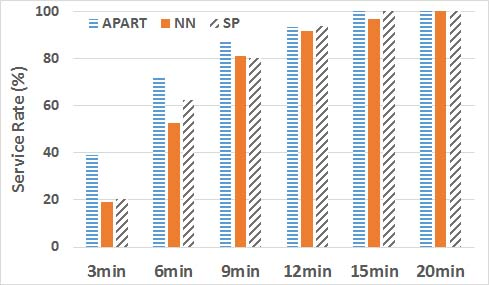
\includegraphics[width = 0.45\columnwidth]{fig/mwt_sr.jpg}
    }
    \subfigure[\small{Number of Drivers}]{
        \label{fig:nd_sr}
        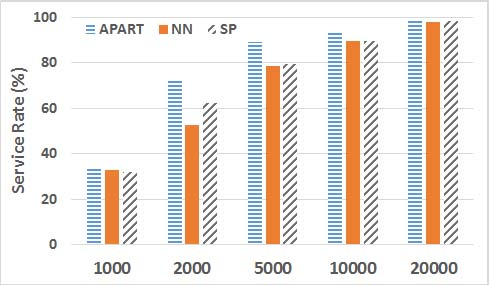
\includegraphics[width = 0.45\columnwidth]{fig/nd_sr.jpg}
    }
    \subfigure[\small{Maximum Passengers}]{
        \label{fig:mp_sr}
        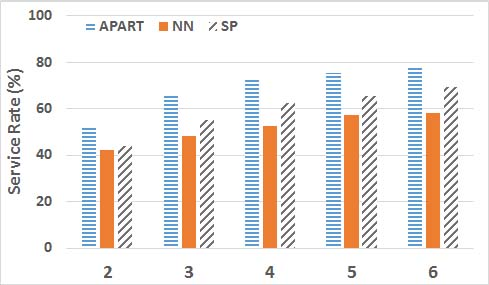
\includegraphics[width = 0.45\columnwidth]{fig/mp_sr.jpg}
    }
    \subfigure[\small{Maximum Allowed Detour}]{
        \label{fig:mad_sr}
        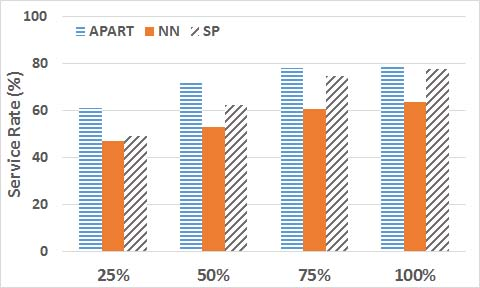
\includegraphics[width = 0.45\columnwidth]{fig/mad_sr.jpg}
    }
    \vspace{-0.15in}
    \caption{Comparing Service Rate of the Algorithms}
    \label{fig:sr}
\end{figure}

\subsubsection{Revenue}
As mentioned, the main objective of APART is to maximize the ridesharing platform's revenue. In these set of experiments, we compare the generated revenue of each algorithm. In these experiments we applied the pricing model explained in \TODO{mohammad}{ref to correct section} and used for the riders and drivers, used profiles similar to the ones in \TODO{mohammad}{ref to sample rider profiles} and \TODO{mohammad}{ref to sample driver profile} respectively. Here, we want to evaluate the effect of varying the parameters in \cref{tab:params} on the overall revenue and compare different algorithms. Later in \cref{subsec:pricingexp} we will apply different pricing models to the algorithms and compare revenue under different pricing models as well.

\begin{figure}[h]
    \centering
    \subfigure[\small{Maximum Wait Time}]{
        \label{fig:mwt_rev}
        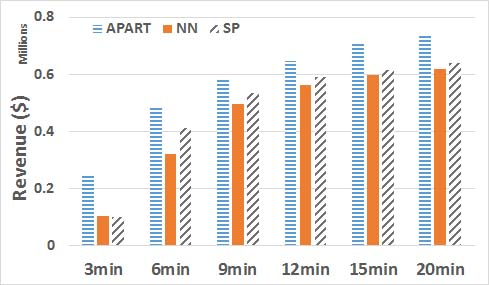
\includegraphics[width = 0.45\columnwidth]{fig/mwt_rev.jpg}
    }
    \subfigure[\small{Number of Drivers}]{
        \label{fig:nd_rev}
        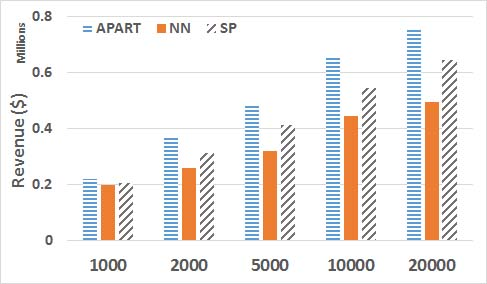
\includegraphics[width = 0.45\columnwidth]{fig/nd_rev.jpg}
    }
    \subfigure[\small{Maximum Passengers}]{
        \label{fig:mp_rev}
        \includegraphics[width = 0.45\columnwidth]{fig/mp_rev.jpg}
    }
    \subfigure[\small{Maximum Allowed Detour}]{
        \label{fig:mad_rev}
        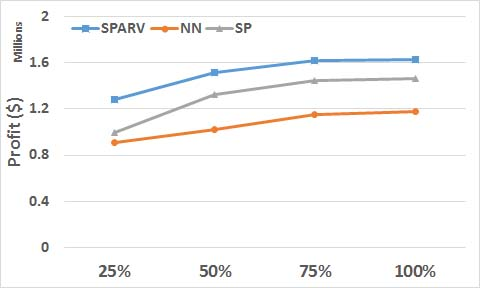
\includegraphics[width = 0.45\columnwidth]{fig/mad_rev.jpg}
    }
    \vspace{-0.15in}
    \caption{Comparing Revenue of the Algorithms}
    \label{fig:rev}
\end{figure}

As it can be seen in \cref{fig:rev} regardless of the values of different parameters, APART generates more revenue than any other approach. When we compare the results in \cref{fig:rev} with the ones in \cref{fig:sr}, even under configurations where all algorithms have the same service rate, APART manages to generate at least 10\% more revenue. The main reason for higher revenue is that APART is designed to make a \textit{Price-aware} assignment, i.e., assign the request to a driver that generates the most profit. Of course, as explained in \TODO{mohammad}{ref to pricing model section}, the pricing models that are used in APART are designed such that the higher profits are not gained by scamming the riders. On the other hand, as it was explained earlier, the SP and NN algorithm were not designed to maximize revenue. An interesting observation in \cref{fig:nd_ref} is that as more drivers are added, the profit decreases even though the service rate increases (\cref{fig:nd_sr}). The NN algorithm gives priority to drivers that are closer to the pick-up location of a request. As long as the driver is able to fit the request in its current schedule without violating the wait time and maximum detour constraints of any request, the request will be assigned to him. This means under certain conditions the sum of discounts other riders will receive can potentially be higher than the final fare of the new request and hence, the system will end up loosing money.

\subsubsection{Response Time}

Similar to \cite{Ma13,Huang14}, APART processes the requests, one request at a time once a request is submitted. In order to evaluate the scalability of our framework, our next set of experiments evaluate the response time of processing a single request. To count for the communication cost of these algorithms, for every message transfer, we add the communication cost as the \textit{message size} divided by a transmission rate of 1Mbit/sec (this is even less than the average speed of a 3G cellular network). \cref{fig:rp} compares the response time of the algorithms under different configurations.

\begin{figure}[h]
    \centering
    \subfigure[\small{Maximum Wait Time}]{
        \label{fig:mwt_rp}
        \includegraphics[width = 0.45\columnwidth]{fig/mwt_rp.jpg}
    }
    \subfigure[\small{Number of Drivers}]{
        \label{fig:nd_rp}
        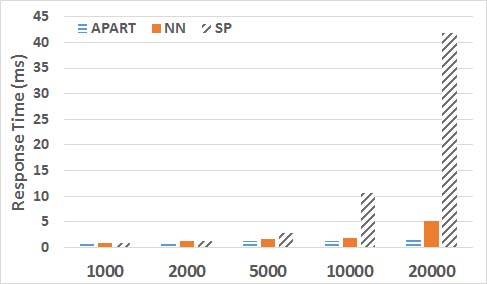
\includegraphics[width = 0.45\columnwidth]{fig/nd_rp.jpg}
    }
    \subfigure[\small{Maximum Passengers}]{
        \label{fig:mp_rp}
        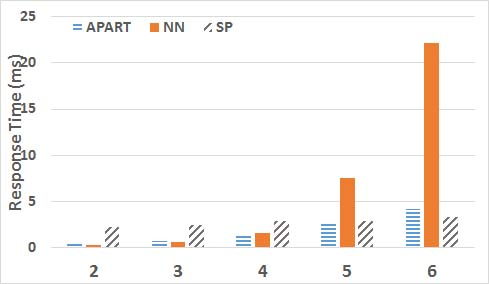
\includegraphics[width = 0.45\columnwidth]{fig/mp_rp.jpg}
    }
    \subfigure[\small{Maximum Allowed Detour}]{
        \label{fig:mad_rp}
        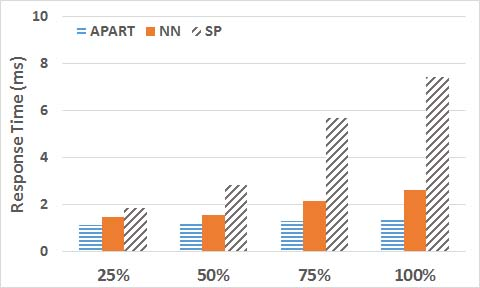
\includegraphics[width = 0.45\columnwidth]{fig/mad_rp.jpg}
    }
    \vspace{-0.15in}
    \caption{Comparing Revenue of the Algorithms}
    \label{fig:rp}
\end{figure}

In \cref{fig:mwt_rp}, the response time increases as more wait time is allowed. This is expected as more wait time, allows drivers to schedule more requests simultaneously which makes the scheduling more time consuming. However, all approaches manage to keep the response time less than 3ms which is acceptable for a real-time framework. However, in \cref{fig:nd_rp}, when more drivers are added, the scalability of SP suffers as it has to perform scheduling for a larger number of vehicles. On the other hand, due to the distributed nature of APART's auction-based approach, each driver does scheduling for itself and adding drivers does not affect the overall response time of APART as much. In \cref{fig:mp_rd} we notice that although APART's response time does not go beyond 2ms, SP handles the increase in maximum passengers better due to the Kinetic Tree structure implementation \cite{Huang14}. The reason for NN's poor performance in \cref{fig:mp_rp} is that it has to \textit{sequentially} perform a computation heavy scheduling, for possibly multiple drivers.

\subsection{Comparing Pricing Models}
\label{subsec:pricingexp}

\section{Related Work}
%In the following, we first review the related work regarding static ridesharing, then discuss real-time ridesharing. Pricing scheme and task assignment and scheduing in spatial crowdsouring.

% offline ridesharing
There are mainly two categories of ridesharing, i.e., static and dyanmic ridesharing. Most existing studies~\cite{FuruhataTRB13, Santi14, CiciUbicom14} belong to static ridesharing, where all riderS and drives are knownn in priori, and thus trips are prearranged. Furuhata et al.~\cite{FuruhataTRB13} provoides a compresensive suvery of the different types of ride sharing regarding their formulations, optimizations and key computations challenges. Santi et al.~\cite{Santi14} proposed a graph-based approach to quantify the potential of ridesharing using NewYork taxi data, and Cici et al.~\cite{CiciUbicom14} evaluated the potential of carpooling using four cities' mobile dataset. In addition, ridesharing problem can be treated as a special class of the dial-a-ride problem (DARP)~\cite{Cordeau07}, or dynamic vehicle routing problem (VRP)~\cite{LiSstd15} in operational research, which is proven to be NP-hard. All these studies assume that the rider and drivers status are know in advance, and hence can afford high computation cost, which is not the case in real-time ridesharing.

% real-time ridesharing
With the emergence of many ridesahring mobile applications (e.g., Uber and Lyft), real-time ridesharing~\cite{Ma13, Ma15, Huang14,OtaBigdata15, CiciGis15, CaoMDM15, PelzerITS15} attracts more research interest recently. Ma et al.~\cite{Ma13, Ma15} proposed a ridesharing dispatch system named ``T-share" to serve the rider request on-the-fly with the objective of reducing driver's total travel distance. Their work focus on maintaining a spatial-temporal indexing to retrieve the candidate drivers. On the other hand, Huang~\cite{Huang14} proposed a kinect tree scheduling algorithm to dynamically match trip request to drivers with minimum incurred travel distance. Ota et al.~\cite{OtaBigdata15} introduced a data-driven simuation framework that enables the analysis of ride-sharing by using NY taxi dataset. Santos et. al~\cite{SantosIjcai13} propose a ride sharing system to maximize the number of matched request. The majority of these studies aim to minimize the total travel distance of drivers, however, we show that this does not necessarily mean shorter travel distance for the riders. Compared with these work, we discuss the conflicting interest between riders, drivers and platform providers. We propose a general and flexible pricing scheme and  our objective is to maximize the total profit of platform. We show that by maximizing the overall profit, our framework achieves higher service rate and quality.  Finally, We introduced a decentralized auction-based framework to support scalable and real-time scheduling, which differs existing centralized scheduling framework. 
%Because of this decentralized framework, the kinect tree scheduling algorithm proposed in Huang~\cite{Huang14} can be easily integrated into APART to purse further efficiency. \dingedit{Do we need this last sentence?}

% pricing scheme
Pricing mechanisms in realtime ridesharing have also been studied in~\cite{KamarIJCAI09,KleinerIJCAI11, ZhaoAAMAS14}. Their main focus is to adapt the well-known VCG mechanism~\cite{Nisan07} for truthful bidding, while addressing the specific challenges such as computational issues, incentive compatibility~\cite{KamarIJCAI09, KleinerIJCAI11} and deficit control~\cite{ZhaoAAMAS14}. These studies are orthogonal to our paper, and can be integrated into our framework APART when we compute the bid of each candidate driver. 

% spatial crowdsourcing
Our work is also related to the task assignment and scheduling problem in spatial crowdsourcing~\cite{KazemiGis12, DengGis13, DengGis15}. Spatial crowdsourcing is a platform, whic enables a requester to comission workers to physically travel to some specified locations to perform a set of spatial tasks. For example, Kazemi et. al~\cite{KazemiGis12} formuated task assignment in spatial crowdsourcing as a min-cost max-flow problem, Deng et. al studied both task scheduling problem for one single worker~\cite{DengGis13} and multiple workers~\cite{DengGis15}. Different with spatial crowdsourcing, in real-time ridesharing, each rider request consists of both pickup and dropoff locations. In addition, their assignment and scheduling are processed in a batch fashion (e.g., batching tasks and workers every 10 minutes), whereas each rider requst in realtime ridesharing must be processed in a short amount of time.

\section{Conclusion}


\section*{Acknowledgement}
This research has been funded in in part by NSF grants IIS-1320149 and CNS-1461963, METRANS Transportation Center under grants from Caltrans (DTRT12-G-UTC57), and the USC Integrated Media Systems Center. Any opinions, findings and conclusions or recommendations expressed in this material are those of the authors and do not necessarily reflect the views of any of the sponsors.

\begin{scriptsize}
\bibliographystyle{acm}
\bibliography{sigproc}
\end{scriptsize}

\end{document}
